%% NOTICE: Overleaf free plan is limiting this compilation, so it is better to compile using your own computer
\documentclass{beamer}

%% TODO: Uncomment the next three lines to add notes to presentation slides
%\usepackage{pgfpages}
%\setbeameroption{show notes on second screen}
%\setbeamertemplate{note page}{\insertnote}

\usepackage[utf8]{inputenc}

\usepackage{graphicx}

%% TODO: Put all the figure files inside the images folder
\graphicspath{{images/}}

\usepackage{amsmath}
\usepackage{amssymb}

\usepackage{pifont}

%% TODO: Use \cmark for tick and \xmark for x
\newcommand{\cmark}{\ding{51}}%
\newcommand{\xmark}{\ding{55}}%

\usepackage{algorithm}
\usepackage{algpseudocode}

%% TODO: Comment the next three lines to remove the bibliography
\usepackage[backend=biber,style=numeric, citestyle=ieee]{biblatex}
\addbibresource{References.bib}
\AtBeginBibliography{\small}

\usepackage{appendixnumberbeamer}
\pdfstringdefDisableCommands{%
\def\translate#1{#1}%
}

%% TODO: Comment the next line if you need the control symbol
\beamertemplatenavigationsymbolsempty

\usetheme{Berlin}
\useinnertheme{circles}

\AtBeginSection[]
{
 \begin{frame}
 \frametitle{Table of Contents}
 \tableofcontents[currentsection]
 \end{frame}
}

%% TODO: Add information to the title page
\title{Code Generation with Vision Language Models for Robot Arms Application}
\author{Tran Quang Minh, Luu Trong Hieu, Nguyen Cong Khanh, Nguyen Quang Trung}
\institute[FPT University - VietDynamic JSC]{
 \textit{Department of Artificial Intelligence} \\
 FPT University - VietDynamic JSC}
\date{Internship Presentation - Fall 2025}

%% Page number
\expandafter\def\expandafter\insertshorttitle\expandafter{%
 \insertshorttitle\hfill%
 \insertframenumber\,/\,\inserttotalframenumber}

\begin{document}

%% Title frame
\begin{frame}
    \titlepage
    \note{This presentation covers our internship work on code generation with VLMs for robot arm applications at VietDynamic JSC from September to December 2025.}
\end{frame}

%% ToC frame
\begin{frame}{Table of Contents}
    \tableofcontents
    \note{Overview of the presentation structure covering introduction, related work, methodology, results, and conclusions.}
\end{frame}

\section{Introduction} 

\begin{frame}{Motivation}
    \begin{itemize} 	
        \item The rapid advancement of \alert{AI and machine learning} has led to development of vision language models (VLMs)
        \item VLMs show remarkable capabilities in \alert{natural language processing tasks}, including code generation
        \item \alert{Automated code generation} has significant implications for software development in robotics
        \item Opportunity to explore VLMs for \alert{robot arm applications} at VietDynamic JSC
    \end{itemize}
    \note{Emphasize the growing importance of AI in robotics and the specific opportunity this internship provided.}
\end{frame}

\begin{frame}[label=objectives]{Project Objectives}
    \begin{block}{Primary Objective}
        Explore the capabilities of \alert{vision language models (VLMs)} in generating code for robot arm applications
    \end{block}
    \begin{block}{Secondary Objectives}
        \begin{itemize}
            \item Automate the coding process for robotics
            \item Improve efficiency and reduce development time
            \item Integrate visual understanding with code generation
            \item Validate generated code in simulation environments
        \end{itemize}
    \end{block}
    \note{These objectives guide the entire project approach and methodology.}
\end{frame}

\begin{frame}{Internship Details}
    \textbf{Duration:} September 2025 - December 2025
    
    \textbf{Location:} VietDynamic JSC, Ho Chi Minh City
    
    \textbf{Team Members:}
    \begin{itemize}
        \item Tran Quang Minh
        \item Luu Trong Hieu  
        \item Nguyen Cong Khanh
        \item Nguyen Quang Trung
    \end{itemize}
    
    \textbf{GitHub Repository:} \url{https://github.com/Minhtrna/Code-gen-for-robot-arm-OJT-FALL-2025-FPT}
    
    \note{Provide context about the internship setting and team composition.}
\end{frame}

\section{Related Work}

\begin{frame}{State of the Art}
    \begin{block}{Key Research Areas}
        \begin{itemize}
            \item \alert{RoboCodeX} \cite{mu2024robocodex}: LLMs for robotic task code generation
            \item \alert{Robotic Programmer} \cite{xie2025robotic}: Video-instructed policy code generation
            \item \alert{MobileVLM} \cite{chu2023mobilevlm}: Multimodal vision-language models
        \end{itemize}
    \end{block}
    
    \begin{alertblock}{Research Gap}
        Integration of \alert{3D visual sensors} with VLMs for industrial robot arm applications remains underexplored
    \end{alertblock}
    
    $\Rightarrow$ \textbf{Our work addresses this gap by combining Mech-EYE 3D cameras with VLMs.}
    
    \note{Highlight how our work builds upon and extends existing research in the field.}
\end{frame}
         
\section{Methodology} 

\begin{frame}{System Overview}
    \begin{figure}
        \centering
        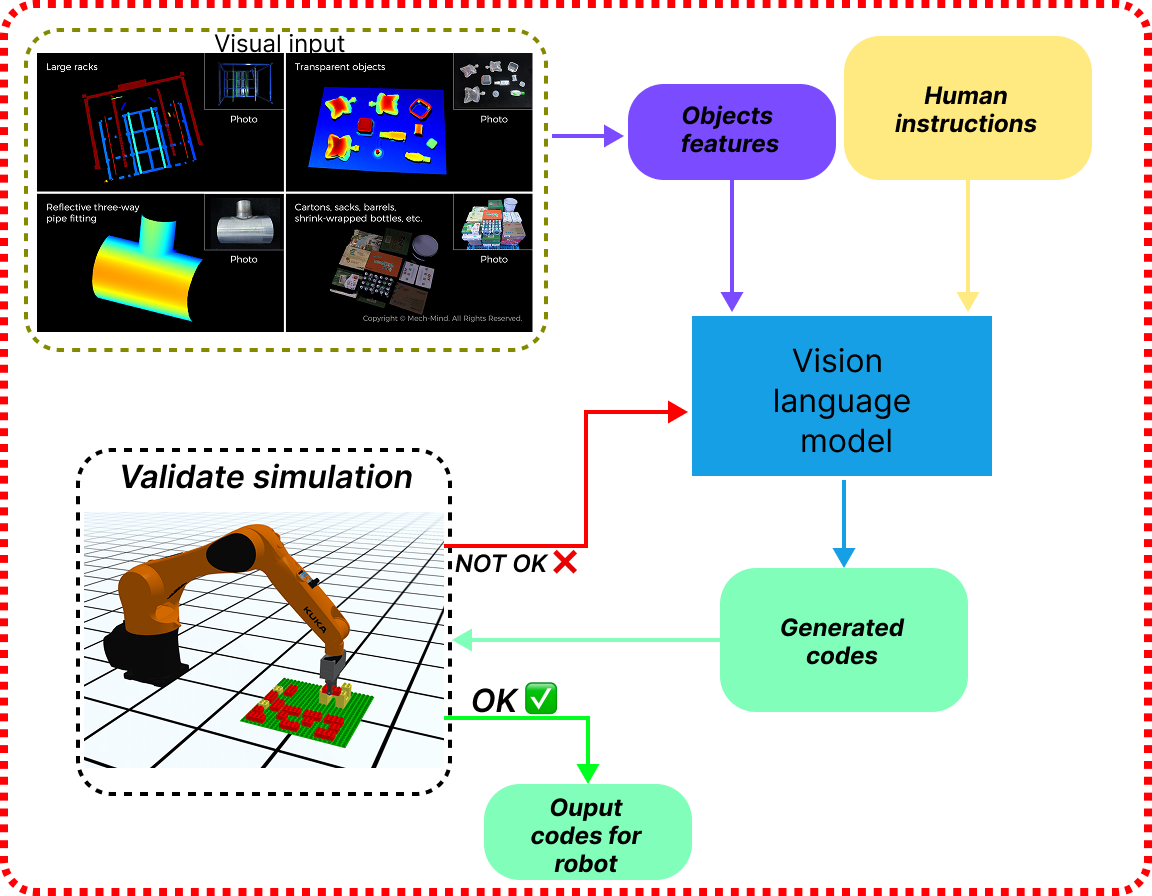
\includegraphics[width=.8\linewidth]{OJT_fig_1.png}
        \caption{Overall pipeline architecture combining 3D vision, VLMs, and simulation validation.}
    \end{figure}	
    \note{This figure shows the complete workflow from visual input to code validation.}
\end{frame}

\begin{frame}{Pipeline Components}
    \begin{columns}
        \column{0.5\textwidth}
        \centering
        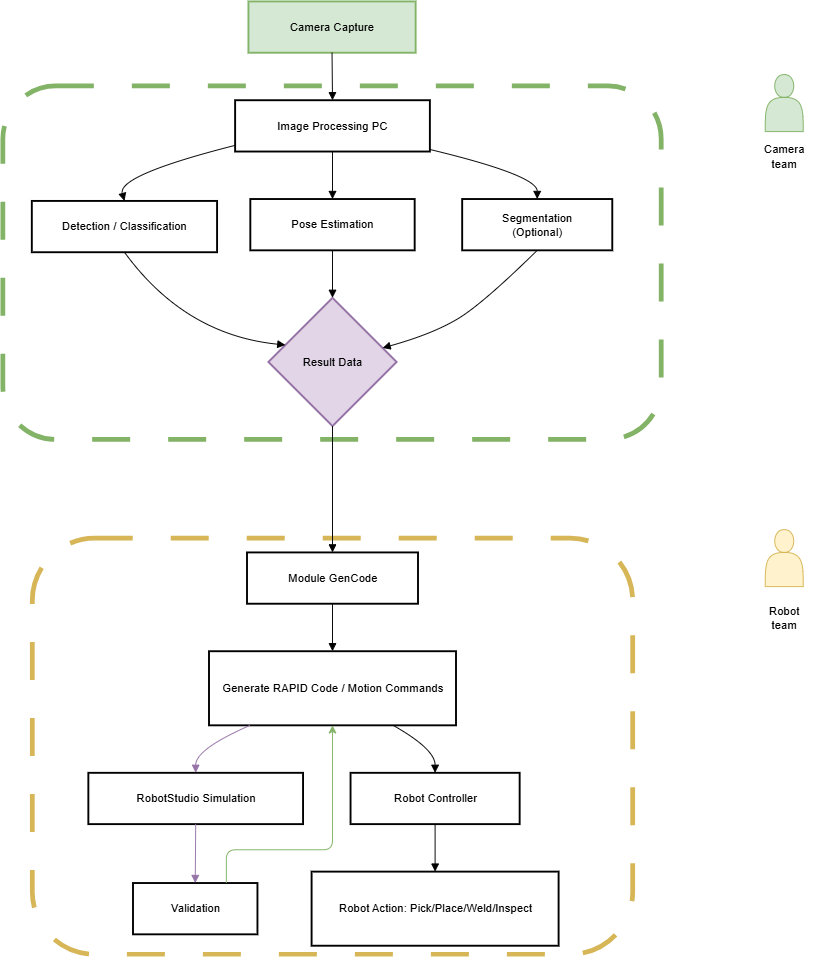
\includegraphics[width=5cm]{flow.png}
        \column{0.5\textwidth}
        \begin{itemize}
            \item \textbf{Mech-EYE 3D Camera:} Captures high-resolution images and 3D point clouds
            \item \textbf{Vision Language Models:} Process visual data and generate robot code
            \item \textbf{ROS2 + Gazebo:} Simulation environment for code validation
            \item \textbf{Integration:} Seamless pipeline from perception to execution
        \end{itemize}
    \end{columns}
    \note{Each component plays a crucial role in the overall system architecture.}
\end{frame}

\begin{frame}{Technical Stack}
    \begin{block}{Hardware Components}
        \begin{itemize}
            \item \alert{Mech-EYE 3D Industrial Camera} - High-precision visual sensing
            \item Robot arm simulation platform
        \end{itemize}
    \end{block}
    
    \begin{block}{Software Framework}
        \begin{itemize}
            \item \alert{ROS2} - Robot Operating System for communication
            \item \alert{Gazebo} - Physics simulation environment  
            \item \alert{Vision Language Models} - MobileVLM, RoboCodeX variants
        \end{itemize}
    \end{block}
    
    \note{This combination provides a robust foundation for development and testing.}
\end{frame}
                                
\section{Results} 
            
\begin{frame}{Current Progress}
    \textbf{GitHub Repository:} \url{https://github.com/Minhtrna/Code-gen-for-robot-arm-OJT-FALL-2025-FPT}
                                                                
    \textbf{Key Achievements:}
    \begin{itemize}
        \item Successfully integrated Mech-EYE 3D camera with ROS2
        \item Developed VLM-based code generation pipeline
        \item Created simulation environment for validation
        \item Established end-to-end workflow
    \end{itemize}
    
    \begin{columns}
        \column{0.5\textwidth}
        \begin{figure}
            \centering
            \fbox{3D Point Cloud Visualization}
            \caption{Mech-EYE camera output}
        \end{figure}	
        \column{0.5\textwidth}
        \begin{figure}
            \centering
            \fbox{Gazebo Simulation}
            \caption{Robot arm simulation}
        \end{figure}
    \end{columns}
    \note{Show concrete progress made during the internship period.}
\end{frame}

\begin{frame}{Technical Contributions}
    \begin{block}{Data Collection Pipeline}
        \begin{itemize}
            \item Automated capture of 3D visual data
            \item Integration with robot workspace mapping
            \item Real-time processing capabilities
        \end{itemize}
    \end{block}
    
    \begin{block}{Code Generation Framework}
        \begin{itemize}
            \item VLM adaptation for robotics domain
            \item Context-aware code generation
            \item Safety constraint integration
        \end{itemize}
    \end{block}
    
    \note{Highlight the specific technical innovations developed during the internship.}
\end{frame}
            
\section{Discussion} 
    
\begin{frame}{Challenges and Limitations}
    \begin{itemize}
        \item \alert{Model Accuracy:} VLMs require fine-tuning for robotics-specific tasks
        \item \alert{Real-time Performance:} Balancing accuracy with processing speed
        \item \alert{Safety Constraints:} Ensuring generated code follows safety protocols
        \item \alert{Hardware Integration:} Synchronizing 3D vision with motion planning
    \end{itemize}
    
    $\Rightarrow$ \textbf{Future work will focus on addressing these technical challenges.}
    
    \note{Be honest about current limitations while showing awareness of solutions.}
\end{frame}

\begin{frame}{Impact and Applications}
    \begin{block}{Industrial Applications}
        \begin{itemize}
            \item Automated assembly line programming
            \item Pick-and-place operation optimization
            \item Quality control integration
        \end{itemize}
    \end{block}
    
    \begin{block}{Research Contributions}
        \begin{itemize}
            \item Novel integration of 3D vision with VLMs
            \item Open-source framework for community use
            \item Validation methodology for generated code
        \end{itemize}
    \end{block}
    
    \note{Emphasize both practical and academic value of the work.}
\end{frame}
                                     
\section{Conclusion}

\begin{frame}{Key Takeaways}
    \begin{block}{Technical Achievements}
        Successfully demonstrated VLM-based code generation for robot arms with 3D visual input
    \end{block}
    
    \begin{block}{Learning Outcomes}
        \begin{itemize}
            \item Deep understanding of vision-language model integration
            \item Practical experience with ROS2 and Gazebo simulation
            \item Industry collaboration skills at VietDynamic JSC
        \end{itemize}
    \end{block}
    
    \begin{alertblock}{Future Directions}
        Real-world deployment and performance optimization
    \end{alertblock}
    
    \note{Summarize the main accomplishments and learning from the internship.}
\end{frame}

\begin{frame}{Acknowledgments}
    \begin{block}{Special Thanks}
        \begin{itemize}
            \item \alert{VietDynamic JSC} for providing this valuable learning opportunity
            \item \alert{FPT University} for academic support and guidance
            \item Internship supervisors and mentors
            \item Team members for collaborative effort
        \end{itemize}
    \end{block}
    
    \textbf{Contact:} 
    \begin{itemize}
        \item quantran102005@gmail.com
        \item Luutronghieu0709@gmail.com  
        \item congkhanhtruongthi@gmail.com
        \item trungnqse183108@fpt.edu.vn
    \end{itemize}
    
    \note{Express gratitude to all parties who made this internship possible.}
\end{frame}
                                                         
%% Thank You frame
\begin{frame}
    \centering
    \Huge Thank You!
    
    \vspace{1cm}
    \Large Questions \& Discussion
    
    \note{Open floor for questions and further discussion about the project.}
\end{frame}
                    
%% Appendix frames
\appendix

\begin{frame}[allowframebreaks, noframenumbering]{References}
    \printbibliography[heading=none]
\end{frame}
                    
\end{document}